%%%%%%%%%%%%%%%%%%%%%%%%%%%%%%%%%%%%%%%%%
% Beamer Presentation
% LaTeX Template
% Version 1.0 (10/11/12)
%
% This template has been downloaded from:
% http://www.LaTeXTemplates.com
%
% License:
% CC BY-NC-SA 3.0 (http://creativecommons.org/licenses/by-nc-sa/3.0/)
%
%%%%%%%%%%%%%%%%%%%%%%%%%%%%%%%%%%%%%%%%%

%----------------------------------------------------------------------------------------
%	PACKAGES AND THEMES
%----------------------------------------------------------------------------------------

\documentclass{beamer}

\mode<presentation> {

% The Beamer class comes with a number of default slide themes
% which change the colors and layouts of slides. Below this is a list
% of all the themes, uncomment each in turn to see what they look like.

%\usetheme{default}
%\usetheme{AnnArbor}
%\usetheme{Antibes}
%\usetheme{Bergen}
%\usetheme{Berkeley}
%\usetheme{Berlin}
%\usetheme{Boadilla}
%\usetheme{CambridgeUS}
%\usetheme{Copenhagen}
%\usetheme{Darmstadt}
%\usetheme{Dresden}
%\usetheme{Frankfurt}
%\usetheme{Goettingen}
%\usetheme{Hannover}
%\usetheme{Ilmenau}
%\usetheme{JuanLesPins}
%\usetheme{Luebeck}
\usetheme{Madrid}
%\usetheme{Malmoe}
%\usetheme{Marburg}
%\usetheme{Montpellier}
%\usetheme{PaloAlto}
%\usetheme{Pittsburgh}
%\usetheme{Rochester}
%\usetheme{Singapore}
%\usetheme{Szeged}
%\usetheme{Warsaw}

% As well as themes, the Beamer class has a number of color themes
% for any slide theme. Uncomment each of these in turn to see how it
% changes the colors of your current slide theme.

%\usecolortheme{albatross}
%\usecolortheme{beaver}
%\usecolortheme{beetle}
%\usecolortheme{crane}
%\usecolortheme{dolphin}
%\usecolortheme{dove}
%\usecolortheme{fly}
%\usecolortheme{lily}
%\usecolortheme{orchid}
%\usecolortheme{rose}
%\usecolortheme{seagull}
%\usecolortheme{seahorse}
%\usecolortheme{whale}
%\usecolortheme{wolverine}

%\setbeamertemplate{footline} % To remove the footer line in all slides uncomment this line
%\setbeamertemplate{footline}[page number] % To replace the footer line in all slides with a simple slide count uncomment this line

%\setbeamertemplate{navigation symbols}{} % To remove the navigation symbols from the bottom of all slides uncomment this line
}

\usepackage{graphicx} % Allows including images
\usepackage{booktabs} % Allows the use of \toprule, \midrule and \bottomrule in tables

%----------------------------------------------------------------------------------------
%	TITLE PAGE
%----------------------------------------------------------------------------------------

\title[Anum - Bilangan dan Galat]{Analisis Numerik\\Representasi Bilangan} % The short title appears at the bottom of every slide, the full title is only on the title page

\author{Ahmad Rio Adriansyah} % Your name
\institute[STT-NF] % Your institution as it will appear on the bottom of every slide, may be shorthand to save space
{
STT Terpadu - Nurul Fikri \\ % Your institution for the title page
\medskip
\textit{ahmad.rio.adriansyah@gmail.com
\\arasy@nurulfikri.ac.id} % Your email address
}
\date{\today} % Date, can be changed to a custom date

\usepackage{graphicx}
\begin{document}

\begin{frame}
\titlepage % Print the title page as the first slide
\end{frame}

%----------------------------------------------------------------------------------------
%	PRESENTATION SLIDES
%----------------------------------------------------------------------------------------

%------------------------------------------------
\begin{frame}
\frametitle{Representasi Bilangan Bulat}
Dalam komputer, bilangan dituliskan dalam bit (binary digit).
\\\ \\Contoh : 13 direpresentasikan dalam 8-bit 
\\\ \\$13_{10} = 00001101_2$ 
\\\qquad  $= 0 x 2^7 + 0 x 2^6 + 0 x 2^5 + 0 x 2^4 +
		     1 x 2^3 + 1 x 2^2 + 0 x 2^1 + 1 x 2^0$
\\\qquad  $= 0 + 0 + 0 + 0 + 8 + 4 + 0 + 1$
\end{frame}

%----------------------------------------------------------------------------------------
\begin{frame}
\frametitle{Binary ke Desimal}
$00001101_2 = \underbrace{0}_{2^7}\underbrace{0}_{2^6}\underbrace{0}_{2^5}\underbrace{0}_{2^4}\underbrace{1}_{2^3}\underbrace{1}_{2^2}\underbrace{0}_{2^1}\underbrace{1}_{2^0}$
\\\ \\\ \\\ \\$2^3+2^2+2^0 = 8+4+1 = 13_{10}$
\end{frame}

%----------------------------------------------------------------------------------------
\begin{frame}
\frametitle{Desimal ke Binary}
\begin{equation}
\begin{split}
13 &= 6 x 2 + 1
\\6 &= 3 x 2 + 0
\\3 &= 1 x 2 + 1 
\\1 &= 0 x 2 + 1 \qquad \uparrow
\end{split}
\nonumber
\end{equation}
\ \\\ \\\ \\Dibaca dari yang paling bawah : $13_{10} = 1101_2$
\\atau...
\end{frame}

%----------------------------------------------------------------------------------------
\begin{frame}
\frametitle{Desimal ke Binary}
\begin{center}
\begin{tabular}{|c|c|c|c|}
\hline
	Nilai $2^n$ & Desimal & Nilai $2^n$ & Desimal\\
\hline
	$2^0$ & 1 & $2^4$ & 16\\
\hline
	$2^1$ & 2 & $2^5$ & 32\\
\hline
	$2^2$ & 4 & $2^6$ & 64\\
\hline
	$2^3$ & 8 & $2^7$ & 128\\
\hline
\end{tabular}
\end{center}
\begin{equation}
\begin{split}
13 - \boxed{8} = 5 &\qquad ;2^3
\\5 - \boxed{4} = 1 &\qquad ;2^2
\\1 - \boxed{1} = 0  &\qquad ;2^0
\end{split}
\nonumber
\end{equation}
\ \\\ \\\ \\Dengan kata lain $13_{10} = 2^3 + 2^2 + 2^0 = \underbrace{1}_{2^3} \underbrace{1}_{2^2} \underbrace{0}_{2^1} \underbrace{1}_{2^0} = 1101_2$
\end{frame}


%----------------------------------------------------------------------------------------

\begin{frame}
\frametitle{Representasi Bilangan Negatif}
\textit{Signed Magnitude}
\\Dalam metode ini, digit paling kiri digunakan sebagai penanda positif dan negatif. (positif sebagai "0" dan negatif sebagai "1")
\\\ \\Contoh :
\\$00001101 = 13$
\\$10001101 = -13$
\\\ \\\ 
\\\ \\\begin{tabular}{cc}
	&\\
	&\\
	&\\
\end{tabular} 


\end{frame}

%------------------------------------------------

\begin{frame}
\frametitle{Representasi Bilangan Negatif}
\textit{Signed Magnitude}
\\Dalam metode ini, digit paling kiri digunakan sebagai penanda positif dan negatif. (positif sebagai "0" dan negatif sebagai "1")
\\\ \\Contoh :
\\$00001101 = 13$
\\$10001101 = -13$
\\\ \\Kekurangan : tidak mendukung operasi aritmatika pada bilangan biner
\\\ \\\begin{tabular}{cc}
	&\\
	&\\
	&\\
\end{tabular} 


\end{frame}

%------------------------------------------------

\begin{frame}
\frametitle{Representasi Bilangan Negatif}
\textit{Signed Magnitude}
\\Dalam metode ini, digit paling kiri digunakan sebagai penanda positif dan negatif. (positif sebagai "0" dan negatif sebagai "1")
\\\ \\Contoh :
\\$00001101 = 13$
\\$10001101 = -13$
\\\ \\Kekurangan : tidak mendukung operasi aritmatika pada bilangan biner
\\\ \\\begin{tabular}{cc}
	$00001101$ & $13$\\
	$10001101$ & $-13$\\
	\hline
	$10011010$ & $-26$\\
\end{tabular} +


\end{frame}

%------------------------------------------------

\begin{frame}
\frametitle{Representasi Bilangan Negatif}
Komplemen 1 (\textit{One's Complement})
\\Dalam metode ini, negatif dari suatu bilangan dinyatakan dengan cara membalik seluruh digitnya, "0" menjadi "1" dan sebaliknya, "1" menjadi "0"
\\\ \\Contoh :
\\$00001101 = 13$
\\$11110010 = -13$
\\\ \\\ 
\\\ 
\\\ 
\\\ \\

\end{frame}

%------------------------------------------------

\begin{frame}
\frametitle{Representasi Bilangan Negatif}
Komplemen 1 (\textit{One's Complement})
\\Dalam metode ini, negatif dari suatu bilangan dinyatakan dengan cara membalik seluruh digitnya, "0" menjadi "1" dan sebaliknya, "1" menjadi "0"
\\\ \\Contoh :
\\$00001101 = 13$
\\$11110010 = -13$
\\\ \\Jika diperhatikan lebih jauh, 
\\$-13 = 11110010 = 242$
\\$242+13 = 255$ (bilangan tertinggi dalam 8 bit) 
\\\ \\Jadi komplemen dari 13 adalah 242

\end{frame}

%------------------------------------------------

\begin{frame}
\frametitle{Representasi Bilangan Negatif}
Komplemen 1 (\textit{One's Complement})
\\\ \\Pada metode ini terdapat 2 buah nol. Komplemen dari $0^+$ (nol positif), $00000000$ adalah $0^-$ (nol negatif), $11111111$
\begin{figure}[htp]
\centering
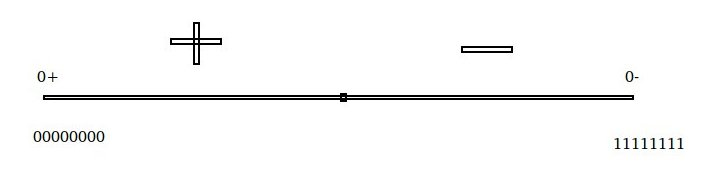
\includegraphics[scale=0.40]{Komp1.jpg}
\end{figure}
Untuk sistem 8 bit, metode ini bisa merepresentasikan -127 s.d. 127
\end{frame}

%------------------------------------------------

\begin{frame}
\frametitle{Representasi Bilangan Negatif}
Komplemen 1 (\textit{One's Complement})
\\\ \\Sebagian masalah terpecahkan. Tapi tetap ada masalah.
\\\ \\Coba jumlahkan $5$ dan $-4$
\\\ \\\begin{tabular}{rc}
	$00000101$ & $5$\\
	$11111011$ & $-4$\\
	\hline
	& \\
\end{tabular} +
\\\ \\\ \\\ \\\ \\ 
\end{frame}

%------------------------------------------------

\begin{frame}
\frametitle{Representasi Bilangan Negatif}
Komplemen 1 (\textit{One's Complement})
\\\ \\Sebagian masalah terpecahkan. Tapi tetap ada masalah.
\\\ \\Coba jumlahkan $5$ dan $-4$
\\\ \\\begin{tabular}{rc}
	$00000101$ & $5$\\
	$11111011$ & $-4$\\
	\hline
	$1.00000000$ & $0$\\
\end{tabular} +
\\\ \\Seharusnya $5-4=1$, tapi dari perhitungan hasilnya 0. SALAH 
\\\ \\Aturan: \\Jika ada nilai pada bit ke-(n+1) setelah \textbf{penjumlahan}, maka harus \textbf{ditambahkan} nilai 1 pada hasilnya.
\\Jika ada nilai pada bit ke-(n+1) setelah \textbf{pengurangan}, maka harus \textbf{dikurangkan} nilai 1 pada hasilnya.
\end{frame}

%------------------------------------------------

\begin{frame}
\frametitle{Representasi Bilangan Negatif}
Komplemen 2 (\textit{Two's Complement})
\\Negatif dari suatu bilangan dinyatakan dengan komplemennya, ditambahkan 1.
\\\ \\Dengan kata lain, "komplemen 2" adalah ("komplemen 1" + 1)
\\\ \\Contoh :
\\$00001101 = 13$
\\$11110010 = -13$ (Komplemen 1)
\\\ \\\begin{tabular}{rcl}
	& & \\
	& & \\
	& & \\
\end{tabular} 


\end{frame}

%------------------------------------------------

\begin{frame}
\frametitle{Representasi Bilangan Negatif}
Komplemen 2 (\textit{Two's Complement})
\\Negatif dari suatu bilangan dinyatakan dengan komplemennya, ditambahkan 1.
\\\ \\Dengan kata lain, "komplemen 2" adalah ("komplemen 1" + 1)
\\\ \\Contoh :
\\$00001101 = 13$
\\$11110010 = -13$ (Komplemen 1)
\\\ \\\begin{tabular}{rcl}
	$11110010$ & $-13$ & (Komplemen 1)\\
	$00000001$ & $1$ & (1 biner)\\
	\hline
	$11110011$ & $-13$ & (Komplemen 2)\\
\end{tabular} +

\end{frame}

%------------------------------------------------

\begin{frame}
\frametitle{Representasi Bilangan Negatif}
Komplemen 2 (\textit{Two's Complement})
\\\ \\\begin{tabular}{rc}
	$00000101$ & $5$\\
	$11111100$ & $-4$\\
	\hline
	$100000001$ & $1$\\
\end{tabular}+
\\\ \\Komplemen 2 menyelesaikan masalah aritmatika binari yang ditemukan pada \textit{signed magnitude} ataupun komplemen 1. Karena itu metode ini yang banyak digunakan pada banyak sistem komputer dewasa ini.
\\\ \\Sistem dengan komplemen 2 sekarang memiliki 1 buah representasi 0. Sistem yang menggunakan 8 bit dapat merepresentasikan bilangan -128 s.d. 127.
\end{frame}

%------------------------------------------------

\begin{frame}
\frametitle{Representasi Bilangan Negatif}
Excess-K :
\\Modifikasi dari Two's Complement
\\Bilangan K disebut nilai bias
\\K (dalam binari Two's Complement) dianggap sebagai angka 0 
\\-K diwakili oleh bilangan yang semua bitnya 0
\\\
\\\
\\Digunakan terutama untuk eksponen dari titik kambang :
\\Single precision (32 bit) = 8 bit excess-127
\\Double precision (64 bit) = 11 bit excess-1023
\\\ 
\\\ 
\\\ 
\\\ 
\end{frame}

%------------------------------------------------

\begin{frame}
\frametitle{Representasi Bilangan Negatif}
Contoh :
\\Excess-128 (8 bit)
\\\ \\\begin{tabular}{|c|c|c|c|}
    \hline
	binari & unsigned & two's complement & excess-128\\
	\hline
	$00000000$ & $0$ & $0$ & $-128$\\
	$00000001$ & $1$ & $1$ & $-127$\\
	$\dots$ & $\dots$ & $\dots$ & $\dots$\\
	$01111111$ & $127$ & $127$ & $-1$\\ 
	$10000000$ & $128$ & $-127$ & $0$\\ 
	$10000001$ & $129$ & $-126$ & $1$\\ 
	$\dots$ & $\dots$ & $\dots$ & $\dots$\\
	$11111110$ & $254$ & $-2$ & $126$\\ 
	$11111111$ & $255$ & $-1$ & $127$\\
	\hline 
\end{tabular}

\end{frame}

%------------------------------------------------

\begin{frame}
\frametitle{Representasi Bilangan Negatif}
Basis (-2)
\\Sama seperti perhitungan biner, tapi basisnya bukan 2, melainkan -2
\\Jadi posisi paling kanan (bit ke-0) mewakili $-2^0 = 1$
\\Bit ke-1 mewakili $-2^1 = -2$
\\Bit ke-$i$ mewakili $-2^i$
\\\ \\
Contoh :
\\00001001 = -7
\\00000110 = 2
\\\ \\\ \\\ \\\ \\\
\end{frame}

%------------------------------------------------

\begin{frame}
\frametitle{Representasi Bilangan Real}
Pada komputer, bilangan real dituliskan dalam bit juga. Untuk mempermudah dalam penalaran, sebagai contoh akan digunakan desimal (basis 10) terlebih dahulu.
\\\ \\Jadi tiap digit dalam komputer diasumsikan dapat diisi angka $0,1,2,...,$ atau $9$, seperti format bilangan yang biasa kita gunakan.
\end{frame}

%----------------------------------------------------------------------------------------
\begin{frame}
\frametitle{Representasi Bilangan Real}
$64636,8968$ bisa dituliskan dalam bentuk 
\begin{equation}
\begin{split}
64&,6368968 \ \ \times 10^3 ,
\\646&,368968 \ \ \ \ \times 10^2 , 
\\0&,646368968 \times 10^5 ,
\\&\text{atau lainnya}
\end{split}
\nonumber
\end{equation}
Bentuk $0,646368968 \times 10^5$ disebut sebagai \underline{bentuk ternormalisasi} atau \underline{bentuk normal}
\end{frame}


%----------------------------------------------------------------------------------------
\begin{frame}
\frametitle{Representasi Bilangan Real}
Bilangan real $254,11377$ dapat dituliskan dalam bentuk normal sebagai 
\begin{equation}
0,25411377 \times 10^3
\nonumber
\end{equation}
Secara umum, bilangan real $a$ dapat dituliskan dalam bentuk
\begin{equation}
a = \pm m \times B^p
\nonumber
\end{equation}
dimana \\$m$ adalah mantisa (nilai "$0,d_1d_2d_3...$" dari bilangan real), \\$B$ adalah basis, dan \\$p$ adalah nilai pangkat dari basisnya
\\\ \\Dalam bentuk normal, digit pertama dari mantisa tidak boleh nol
\end{frame}

%----------------------------------------------------------------------------------------
\begin{frame}
\frametitle{Representasi Bilangan Real}
Dalam komputer, bilangan real disimpan dalam bentuk titik-kambang (\textit{floating point}). 
\\Penyimpanannya dalam bentuk data dibagi menjadi 3 bagian, yaitu "tanda", "pangkat", dan "mantisa"
\begin{figure}[htp]
\centering
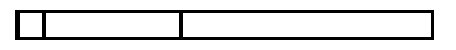
\includegraphics[scale=0.50]{float.jpg}
\end{figure}
\ \\tanda (+ atau -)
\\pangkat ($p$)
\\mantisa ($m$) = angka-angka di belakang koma 
\\\ \\$254,11377 = 0,25411377 \times 10^3$ di dalam \textit{floating point} dituliskan sebagai 
\begin{center}
\begin{tabular}{|c|c|c|}
\hline
	$+$ & $3$ & $25411377$\\
\hline
\end{tabular}
\end{center}
\end{frame}

%----------------------------------------------------------------------------------------
\begin{frame}
\frametitle{Representasi Bilangan Real}
Contoh Lain :
\\\ \\$354860,206 = 0,345860206 \times 10^6$ di dalam bentuk \textit{floating point} dituliskan sebagai 
\begin{center}
\begin{tabular}{|c|c|c|}
\hline
	$+$ & $6$ & $345860206$\\
\hline
\end{tabular}
\end{center}
\ \\\ \\$0,004849458 = 0,4849458 \times 10^{-2}$ di dalam bentuk \textit{floating point} dituliskan sebagai 
\begin{center}
\begin{tabular}{|c|c|c|}
\hline
	$+$ & $-2$ & $4849458$\\
\hline
\end{tabular}
\end{center}
\ \\\ \\$-29,7767025 = -0,297767025 \times 10^{2}$ di dalam bentuk \textit{floating point} dituliskan sebagai 
\begin{center}
\begin{tabular}{|c|c|c|}
\hline
	$-$ & $2$ & $297767025$\\
\hline
\end{tabular}
\end{center}
\end{frame}

%----------------------------------------------------------------------------------------
\begin{frame}
\frametitle{Representasi Bilangan Real}
Dalam komputer, penyimpanan data tidak dapat menggunakan desimal, tetapi binari. Prinsip yang digunakan sama. 
\\\ \\Contoh : bilangan $13,625$ diubah dalam bentuk binari
\begin{equation}
\begin{split}
13,625_{10} &=8+4+1+0,5+0,125 
\\&=2^3+2^2+2^0 + 2^{-1}+2^{-3}
\\&=1101,101_{2}
\\&=0,1101101 \times 2^{4}
\end{split}
\nonumber
\end{equation}
dituliskan dalam bentuk \textit{floating point} sebagai
\begin{center}
\begin{tabular}{|c|c|c|}
\hline
	$+$ & $100$ & $1101101$\\
\hline
\end{tabular}
\end{center}
\end{frame}

%----------------------------------------------------------------------------------------
\begin{frame}
\frametitle{Representasi Bilangan Real}
Pada prakteknya, modifikasi dilakukan untuk mempermudah perhitungan dan menghemat tempat penyimpanan (\textit{storage}) pada memori. Misalnya :
\begin{itemize}
\item Tanda $+$ disimbolkan dengan 0 dan $-$ disimbolkan dengan $1$ 
\item Nilai pangkat positif dan negatif disimbolkan dengan binari \\(misal $3$ disimbolkan dengan $00000010$ dan $-3$ disimbolkan dengan $11111110$)
\item Dalam bentuk normal, digit pertama pasti 1. Digit ini tidak disimpan untuk menghemat 1 bit penyimpanan.
\end{itemize}
Tetapi pada kuliah ini, kita tetap menggunakan tanda $+$ dan $-$, serta semua mantisa dituliskan. Sama seperti contoh.
\end{frame}

%----------------------------------------------------------------------------------------
\begin{frame}
\frametitle{Representasi Bilangan Real}
\begin{center}
\begin{tabular}{|c|c|c|c|}
\hline
	Nilai $2^n$ & Desimal & Nilai $2^n$ & Desimal\\
\hline
	$2^{0}$ & 1 & $2^{-4}$ & 0,0625\\
\hline
	$2^{-1}$ & 0,5 & $2^{-5}$ & 0,03125\\
\hline
	$2^{-2}$ & 0,25 & $2^{-6}$ & 0,015625\\
\hline
	$2^{-3}$ & 0,125 & $2^{-7}$ & 0,0078125\\
\hline
\end{tabular}
\end{center}
\end{frame}


%----------------------------------------------------------------------------------------
\begin{frame}
\frametitle{Representasi Bilangan Real}
Contoh : bilangan $5,7890625$ diubah dalam bentuk binari\\\ \\
\begin{tabular}{ll}
$5,7890625 - \boxed{4} = 1,7890625 $&$;2^{2}$
\\$1,7890625 - \boxed{1} = 0,7890625 $&$;2^{0}$
\\$0,7890625 - \boxed{0,5} = 0,2890625 $&$;2^{-1}$
\\$0,2890625 - \boxed{0,25} = 0,0390625 $&$;2^{-2}$
\\$0,0390625 - \boxed{0,03125} = 0,0078125 $&$;2^{-5}$
\\$0,0078125 - \boxed{0,0078125} = 0 $&$;2^{-7}$
\end{tabular}
\begin{equation}
\begin{split}
5,7890625_{10}&=2^2+2^0+2^{-1}+2^{-2}+2^{-5}+2^{-7} 
\\&= 101,1100101_2 = 0,1011100101 \times 2^3 \qquad \qquad \qquad
\end{split}
\nonumber
\end{equation}
Dituliskan dalam bentuk \textit{floating point} sebagai
\begin{center}
\begin{tabular}{|c|c|c|}
\hline
	$+$ & $11$ & $1011100101$\\
\hline
\end{tabular}
\end{center}
\end{frame}


%----------------------------------------------------------------------------------------
\begin{frame}
\frametitle{Representasi Bilangan Real}
Contoh : bilangan $-7,6875$ diubah dalam bentuk binari\\\ \\
\begin{tabular}{ll}
$7,6875 - \boxed{4} = 3,6875 $&$;2^{2}$
\\$3,6875 - \boxed{2} = 1,6875 $&$;2^{1}$
\\$1,6875 - \boxed{1} = 0,6875 $&$;2^{0}$
\\$0,6875 - \boxed{0,5} = 0,1875 $&$;2^{-1}$
\\$0,1875 - \boxed{0,125} = 0,0625 $&$;2^{-3}$
\\$0,0625 - \boxed{0,0625} = 0 $&$;2^{-4}$
\end{tabular}
\begin{equation}
\begin{split}
-7,6875_{10}&=-(2^2+2^1+2^0+2^{-1}+2^{-3}+2^{-4})
\\&= -111,1011_2 = -0,1111011 \times 2^3 \qquad \qquad \qquad
\end{split}
\nonumber
\end{equation}
Dituliskan dalam bentuk \textit{floating point} sebagai
\begin{center}
\begin{tabular}{|c|c|c|}
\hline
	$-$ & $11$ & $1111011$\\
\hline
\end{tabular}
\end{center}
\end{frame}


%----------------------------------------------------------------------------------------
\begin{frame}
\frametitle{Representasi Bilangan Real}
Contoh : bilangan $0,28125$ diubah dalam bentuk binari\\\ \\
\begin{tabular}{ll}
$0,28125 - \boxed{0,25} = 0,03125 $&$;2^{-2}$
\\$0,03125 - \boxed{0,03125} = 0 $&$;2^{-5}$
\end{tabular}
\begin{equation}
\begin{split}
0,28125_{10}&=2^{-2}+2^{-5}
\\&= 0,01001_2 = 0,1001 \times 2^{-1} \qquad \qquad \qquad
\end{split}
\nonumber
\end{equation}
Dituliskan dalam bentuk \textit{floating point} sebagai
\begin{center}
\begin{tabular}{|c|c|c|}
\hline
	$+$ & $-1$ & $1001$\\
\hline
\end{tabular}
\end{center}
\end{frame}

%----------------------------------------------------------------------------------------
\begin{frame}
\frametitle{Representasi Bilangan Real}
Banyak digit yang digunakan masing-masing bagian dalam \textit{floating point} tergantung kepada jenis komputer (\textit{hardware}) dan kompiler yang dipakai.
\\\ \\Menurut IEEE-754 (sebuah standard teknis untuk komputasi \textit{floating point}), format yang digunakan dalam basis 2 adalah 
\\\begin{center}\begin{tabular}{|c|c|c|c|c|c|}
\hline
	Nama & Nama & Bit & Bit & Digit & Pangkat \\
	&Umum& Mantisa & Pangkat &Desimal &Desimal\\
\hline
	binary16 & Half & 10 & 5  & 3,31 & 4,51 \\
	&Precision&&$-14 \sim 15$&&\\
\hline
	binary32 & Single & 23 & 8 & 7,22 & 38,23 \\
	&Precision&&$-126\sim 127$&&\\
\hline
	binary64 & Double  & 52 & 11  & 15,95 & 307,95 \\
	&Precision&& $-1022\sim 1023$ &&\\
\hline
	binary128 & Quadruple & 112 & 15  & 34,02 & 4931,77 \\
	&Precision&&&&\\
\hline
\end{tabular}
\end{center}

\end{frame}

%----------------------------------------------------------------------------------------
\begin{frame}
\frametitle{Representasi Bilangan Real}
Bit-bit yang digunakan untuk mantisa dan pangkat dapat diperluas sesuai kebutuhan 
\begin{itemize}
\item Semakin tinggi bit pangkatnya, semakin tinggi bilangan yang bisa diwakilkan 
\item Semakin tinggi bit mantisanya, semakin teliti bilangan tersebut diwakilkan (presisinya semakin tinggi)
\end{itemize}
\end{frame}

%----------------------------------------------------------------------------------------
\begin{frame}
\frametitle{Float Converter}
Konverter berikut dapat digunakan untuk meningkatkan pemahaman bagaimana sebuah bilangan dikonversi dalam bit dan seberapa besar error yang dihasilkannya.
\\\ \\
https://www.h-schmidt.net/FloatConverter/IEEE754.html
\end{frame}

%----------------------------------------------------------------------------------------

\begin{frame}
\frametitle{Resume}
\begin{enumerate}
\item Bilangan dituliskan pada komputer dalam bentuk biner (\textit{binary})
\item Bilangan bulat (integer) dituliskan sesuai nilai binernya
\item Bilangan rill (real) dituliskan dalam bentuk ternormalisasi
\begin{equation}
a = \pm m \times B^p
\nonumber
\end{equation}
dan disimpan dalam bentuk titik kambang (\textit{floating point})
\begin{center}
\begin{tabular}{|c|c|c|}
\hline
	$\pm$ & $p$ & $m$\\
\hline
\end{tabular}
\end{center}

\end{enumerate}
\end{frame}

%------------------------------------------------

\begin{frame}
\frametitle{Aritmatika Pada Floating Point}
Bagaimana menjumlahkan $15,912$ dan $1131,8$?
\\\ \\\ 
\\\ \\\begin{tabular}{rl}
	& \\
	& \\
	& \\
\end{tabular}
\\\ \\\ 
\\\ \\\begin{tabular}{rl}
	& \\
	& \\
	& \\
\end{tabular}

\end{frame}

%------------------------------------------------

\begin{frame}
\frametitle{Aritmatika Pada Floating Point}
Bagaimana menjumlahkan  $15,912$ dan $1131,8$?
\\\ \\Keduanya direpresentasikan dalam bentuk ternormalisasi
\\\ \\\begin{tabular}{rl}
	$0,15912$ & $\times 10^2$\\
	$0,11318$ & $\times 10^4$\\
	\hline
	& \\
\end{tabular}+
\\\ \\\ \\\
\\\ \\\begin{tabular}{rl}
	& \\
	& \\
	& \\
\end{tabular}
\end{frame}

%------------------------------------------------

\begin{frame}
\frametitle{Aritmatika Pada Floating Point}
Bagaimana menjumlahkan  $15,912$ dan $1131,8$?
\\\ \\Keduanya direpresentasikan dalam bentuk ternormalisasi
\\\ \\\begin{tabular}{rl}
	$0,15912$ & $\times 10^2$\\
	$0,11318$ & $\times 10^4$\\
	\hline
	& \\
\end{tabular}+
\\\ \\Sebelum dijumlahkan, perlu dilakukan pergeseran digit untuk menyamakan pangkat
\\\ \\\begin{tabular}{ll}
	$0,0015912$ & $\times 10^4$\\
	$0,11318$ & $\times 10^4$\\
	\hline
	& \\
\end{tabular}+
\end{frame}

%------------------------------------------------

\begin{frame}
\frametitle{Aritmatika Pada Floating Point}
Bagaimana menjumlahkan  $15,912$ dan $1131,8$?
\\\ \\Keduanya direpresentasikan dalam bentuk ternormalisasi
\\\ \\\begin{tabular}{rl}
	$0,15912$ & $\times 10^2$\\
	$0,11318$ & $\times 10^4$\\
	\hline
	& \\
\end{tabular}+
\\\ \\Sebelum dijumlahkan, perlu dilakukan pergeseran digit untuk menyamakan pangkat
\\\ \\\begin{tabular}{ll}
	$0,0015912$ & $\times 10^4$\\
	$0,11318$ & $\times 10^4$\\
	\hline
	$0,1147712$ & $\times 10^4$\\
\end{tabular}+
\end{frame}

%------------------------------------------------

\begin{frame}
\frametitle{Aritmatika Pada Floating Point}
Jika digunakan komputer dengan mantis 5 digit (basis 10), maka hasil penjumlahannya akan terkena galat pembulatan di digit ke-6 dan seterusnya.
\\\ \\$0,1147712\times 10^4\qquad \longrightarrow\qquad 0,11477\times 10^4 \quad+\quad 0,0000012 \times 10^4$
\\\ \\Yang akan disimpan adalah $0,11477\times 10^4$ 
\\dengan galat pembulatan sebesar $\epsilon=0,0000012 \times 10^4$
\end{frame}

%------------------------------------------------

\begin{frame}
\frametitle{Aritmatika Pada Floating Point}
Bagaimana menjumlahkan $3542,99911123$ dan $0,00088877$?
\\\ \\\ 
\\\ \\\begin{tabular}{rl}
	& \\
	& \\
	& \\
\end{tabular}

\end{frame}

%------------------------------------------------

\begin{frame}
\frametitle{Aritmatika Pada Floating Point}
Bagaimana menjumlahkan $3542,99911123$ dan $0,00088877$?
\\\ \\Keduanya direpresentasikan dalam bentuk ternormalisasi
\\\ \\\begin{tabular}{rl}
	$0,354299911123$ & $\times10^4$\\
	$0,88877$ & $\times10^{-3}$\\
	\hline
	??? & ??\\
\end{tabular}+

\end{frame}

%------------------------------------------------

\begin{frame}
\frametitle{Aritmatika Pada Floating Point}
Kalau digunakan komputer dengan mantis 5 digit (basis 10), terdapat galat pembulatan di digit ke-6 dan seterusnya. 
\\\ \\Pembulatannya bisa berupa :
\begin{enumerate}
\item Pemenggalan (\textit{chopping})
\\Digit yang tidak dapat disimpan dalam memori dihilangkan sama sekali
\item Pembulatan (\textit{in-rounding})
\\Digit yang tidak dapat disimpan dalam memori dibulatkan ke digit terdekat
\\$0,1,2,3,4$ dibulatkan ke bawah pada digit sebelah kirinya
\\$5,6,7,8,9$ dibulatkan ke atas pada digit sebelah kirinya
\end{enumerate}              
\end{frame}

%------------------------------------------------

\begin{frame}
\frametitle{Aritmatika Pada Floating Point}
Pembulatan dengan \textit{chopping} 
\\\ \\\begin{tabular}{rl}
	$0,35429$ & $\times10^4$\\
	$0,88877$ & $\times10^{-3}$\\
	\hline
	??? & ??\\
\end{tabular}+
\\\ \\Dan pada saat pergeseran digit untuk menyamakan pangkat, bilangan yang kecil tidak masuk ke dalam perhitungan
\\\ \\\begin{tabular}{ll}
	$0,35429$ & $\times10^4$\\
	$0,000000088877$ & $\times10^{4}$\\
	\hline
	$0,354290088877$ & $\times10^4$\\
\end{tabular}+
\\\ \\Galat pembulatannya $0,000009911123\times10^4$ dari penyimpanan bilangan pertama dan $0,000000088877\times10^{4}$ dari hasil penjumlahannya.
\end{frame}

%------------------------------------------------

\begin{frame}
\frametitle{Aritmatika Pada Floating Point}
Galat pembulatannya $0,000009911123\times10^4$ dari penyimpanan bilangan pertama dan $0,000000088877\times10^{4}$ dari hasil penjumlahannya.
\\\ \\Total galatnya $0,00001\times 10^{4}$

\end{frame}

%------------------------------------------------

\begin{frame}
\frametitle{Aritmatika Pada Floating Point}
Pembulatan dengan \textit{in-rounding} 
\\\ \\$0,354299911123\times10^4$ dibulatkan menjadi $0,35430\times10^4$
\\\ \\\begin{tabular}{rl}
	$0,35430$ & $\times10^4$\\
	$0,88877$ & $\times10^{-3}$\\
	\hline
	??? & ??\\
\end{tabular}+
\\\ \\Pada saat pergeseran digit untuk menyamakan pangkat, bilangan yang kecil tidak masuk ke dalam perhitungan
\\\ \\\begin{tabular}{ll}
	$0,35430$ & $\times10^4$\\
	$0,000000088877$ & $\times10^{4}$\\
	\hline
	$0,354300088877$ & $\times10^4$\\
\end{tabular}+
\\\ \\Galat pembulatannya $-0,000000088877\times10^4$ dari penyimpanan bilangan pertama dan $0,000000088877\times10^{4}$ dari penjumlahannya.
\end{frame}

%------------------------------------------------

\begin{frame}
\frametitle{Aritmatika Pada Floating Point}
Galat pembulatannya $-0,000000088877\times10^4$ dari penyimpanan bilangan pertama dan $0,000000088877\times10^{4}$ dari penjumlahannya.
\\\ \\Total galatnya $0,0\times 10^{4}$. 
\\Dengan kata lain, nilai yang diperoleh sama persis dengan nilai yang sebenarnya.

\end{frame}

%------------------------------------------------

\begin{frame}
\frametitle{Epsilon Mesin}
Jumlah bit yang digunakan untuk representasi bilangan rill terbatas, berarti banyaknya bilangan rill yang bisa direpresentasikan juga terbatas. (seperti kasus bilangan bulat 8 bit hanya dapat merepresentasikan bilangan -128 s.d. 127)
\\\ \\Jika kita punya sistem bilangan \textit{floating point} dengan 6 bit (1 bit untuk tanda, 3 bit untuk pangkat, dan 2 bit mantisa) dan pangkat yang mungkin dari $-2$ s.d. $3$, bilangan yang mungkin dibentuk adalah
\begin{equation}
\pm 0.10 \times 2^p \text{ atau } \pm 0.11 \times 2^p,\text{ dimana } -2 \leq p \leq 3
\nonumber
\end{equation}
\end{frame}

%------------------------------------------------

\begin{frame}
\frametitle{Epsilon Mesin}
\begin{equation}
\pm 0.10 \times 2^p \text{ atau } \pm 0.11 \times 2^p,\text{ dimana } -2 \leq p \leq 3
\nonumber
\end{equation}
\begin{figure}[htp]
\centering
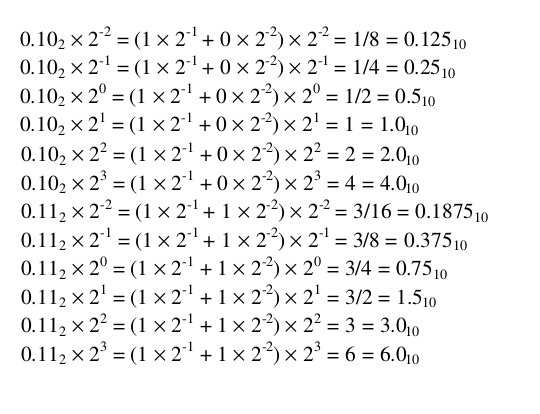
\includegraphics[scale=0.50]{6bit.jpg}
\end{figure}
\end{frame}

%------------------------------------------------

\begin{frame}
\frametitle{Epsilon Mesin}
Floating point berketelitian tunggal (\textit{float}) dinyatakan dalam 32-bit (1 bit tanda, 8 bit pangkat, dan 23 bit mantisa)
\begin{figure}[htp]
\centering
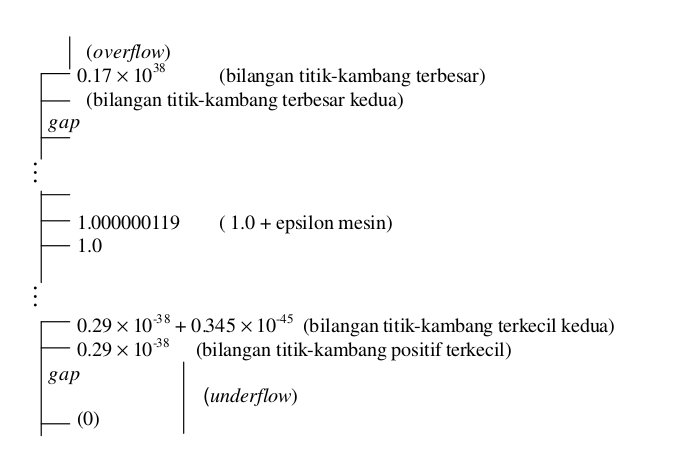
\includegraphics[scale=0.40]{32bit.jpg}
\end{figure}
\end{frame}

%------------------------------------------------

\begin{frame}
\frametitle{Epsilon Mesin}
Epsilon mesin adalah selisih dua buah nilai sangat kecil yang masih dapat dikenali oleh komputer sehingga nilai yang lebih kecil dari itu dianggap nol.
\\\ \\Distandardisasi sebagai bilangan terkecil yang jika ditambahkan dengan 1 memberikan hasil yang lebih besar dari 1.
\begin{equation}
1+\epsilon > 1
\nonumber
\end{equation}
Dalam sistem 32-bit di slide sebelumnya, nilai epsilon mesin adalah $0,000000119$, yaitu $0,119\times 10^{-6}$
\end{frame}

%------------------------------------------------

\begin{frame}
\frametitle{Epsilon Mesin}
Nilai epsilon mesin dapat berbeda-beda tergantung bahasa pemprograman dan komputer yang digunakan. Juga tergantung tipe datanya.
\\\ \\Terkadang ada beberapa bahasa yang menggunakan bilangan berketelitian ganda (\textit{double precision} atau \textit{double})
\\\ \\Epsilon mesin dimanfaatkan sebagai kriteria henti kekonvergenan pada iterasi. Jika galat relatif sudah lebih kecil dari epsilon, iterasi diberhentikan (perhitungan sudah konvergen), jika tidak, iterasi diteruskan.
\end{frame}

%------------------------------------------------

\begin{frame}
\frametitle{Epsilon Mesin}
Cara mencari epsilon mesin 
\begin{figure}[htp]
\centering
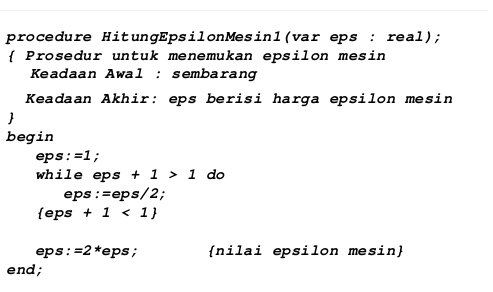
\includegraphics[scale=0.50]{epsilon.jpg}
\end{figure}
\end{frame}

%------------------------------------------------

\begin{frame}
\frametitle{Tugas : Epsilon Mesin}
Buat sebuah program (boleh berbentuk skrip python, C++, java, atau yang lainnya) untuk mencari epsilon mesin.
\end{frame}

%------------------------------------------------

\end{document} 